%%%%%%%%%%%%%%%%%%%%%%%%%%ch3-3
\begin{frame}[shrink]
  \frametitle{ch3.信号检测与估计理论的基础知识}
  \framesubtitle{ch3-3. 贝叶斯准则---例题(续)及性能分析}
  \tableofcontents[hideallsubsections]
\end{frame}

\section{贝叶斯检测步骤回顾}

\begin{frame}
\begin{columns}
	\column{0.5\textwidth}
	\begin{align*}
	&H_0: x=-A+n,\quad H_1: x=A+n\\
	&H_0: x_k=-A+n_k,\quad H_1: x_k=A+n_k\\
	&k=1,2,\dots,N,\quad \bm{x}=(x_1,x_2,\dots,x_N)^{T}\\
	&P(H_i|H_j)=\int_{R_i}p(\bm{x}|H_j)d\bm{x}
	\end{align*}
	\column{0.5\textwidth}
	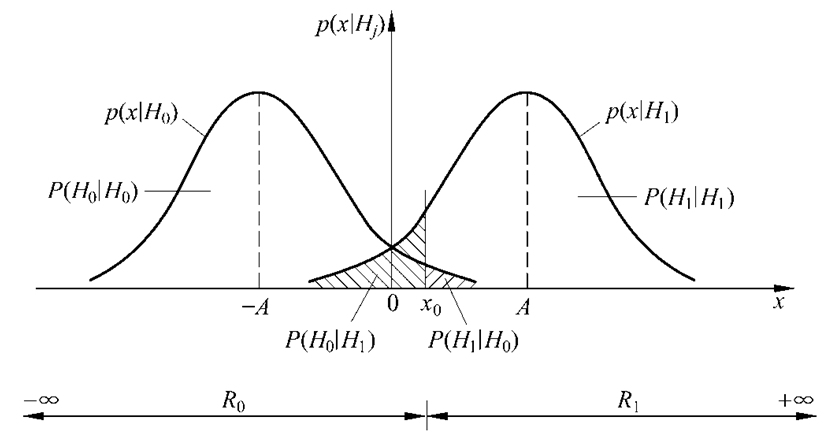
\includegraphics[scale=0.4]{detectionA}
\end{columns}
\begin{align*}
&P(H_0|H_0)=\int_{R_0}p(\bm{x}|H_0)d\bm{x},\qquad P(H_1|H_0)=\int_{R_1}p(\bm{x}|H_0)d\bm{x}\\
&P(H_0|H_1)=\int_{R_0}p(\bm{x}|H_1)d\bm{x},\qquad P(H_1|H_1)=\int_{R_1}p(\bm{x}|H_1)d\bm{x}\\
&\bm{R}=R_0\cup R_1,\quad R_0\cap R_1=\emptyset, \quad \int_{\bm{R}}p(\bm{x}|H_j)d\bm{x}=1\\
&P(H_0|H_0)+P(H_1|H_0)=\int_{R_0}p(\bm{x}|H_0)d\bm{x}+\int_{R_1}p(\bm{x}|H_0)d\bm{x}=\int_{\bm{R}}p(\bm{x}|H_0)d\bm{x}=1\\
&P(H_0|H_1)+P(H_1|H_1)=\int_{R_0}p(\bm{x}|H_1)d\bm{x}+\int_{R_1}p(\bm{x}|H_1)d\bm{x}=\int_{\bm{R}}p(\bm{x}|H_1)d\bm{x}=1
\end{align*}
\end{frame}

\begin{frame}{贝叶斯检测步骤}
\begin{block}{贝叶斯判决准则}
\[ \frac{p(x|H_1)}{p(x|H_0)}\mathop{\gtrless}_{H_0}^{H_1}\frac{P(H_0)(c_{10}-c_{00})}{P(H_1)(c_{01}-c_{11})} \implies \lambda(x)\mathop{\gtrless}_{H_0}^{H_1}\eta \]
\end{block}
利用贝叶斯判决准则进行检测的基本步骤:
\begin{enumerate}
\item 计算两个似然函数, 构建似然比$\lambda(x)\mathop{=}\limits^{def}\frac{p(x|H_1)}{p(x|H_0)}$
\item 根据两个假设的先验概率和代价因子, 计算判决门限$\eta\mathop{=}\limits^{def}\frac{P(H_0)(c_{10}-c_{00})}{P(H_1)(c_{01}-c_{11})}$
\item 利用上式, 形成贝叶斯检测基本表达式$\lambda(x)\mathop{\gtrless}\limits_{H_0}^{H_1}\eta$
\item 化简, 形成贝叶斯检测判决表达式。 如对数似然比检验$\ln\lambda(x)\mathop{\gtrless}\limits_{H_0}^{H_1}\ln\eta\implies l(x)\mathop{\gtrless}\limits_{H_0}^{H_1}\gamma$
\end{enumerate}
\end{frame}

\section{贝叶斯准则例题}

\begin{frame}{贝叶斯准则例题2}
考虑以下信号检测问题:
\begin{align*}
H_0: x_k=n_{0k}, \qquad k=1,2,\dots,N\\
H_1: x_k=n_{1k}, \qquad k=1,2,\dots,N
\end{align*}
其中$n_{0k}$是均值为零,方差为$\sigma_0^2$的高斯随机变量, $n_{1k}$是均值为零,方差为$\sigma_1^2$的高斯随机变量,  且不同采样时刻的加性噪声之间是相互统计独立的。\\
~\\
求: 请给出上述问题的贝叶斯检测准则。
\end{frame}

\begin{frame}[shrink]{贝叶斯准则例题2: 解}
解: $N$次独立采样, 样本为$x_k(k=1,2,\cdots,N)$:
\begin{align*}
H_0: x_k&=n_{0k} && k=1,2,\cdots,N\\
H_1: x_k&=n_{1k} && k=1,2,\cdots,N
\end{align*}
\textbf{步骤1: 计算两个似然函数, 构建似然比}\\
由于$n$是高斯分布随机变量, 因此在$H_0$假设下, 第$k$次采样值$x_k$服从高斯分布,且均值为0, 方差为$\sigma_0^2$; 在$H_1$假设下, 第$k$次采样值$x_k$服从均值为0, 方差为$\sigma_1^2$的高斯分布。
\begin{align*}
p(x_k|H_0)&=\left(\frac{1}{2\pi\sigma_0^2}\right)^{1/2}\exp\left(-\frac{x_k^2}{2\sigma_0^2}\right)\implies p(\bm{x}|H_0)=\prod_{k=1}^{N}\left(\frac{1}{2\pi\sigma_0^2}\right)^{1/2}\exp\left(-\frac{x_k^2}{2\sigma_0^2}\right)\\
p(x_k|H_1)&=\left(\frac{1}{2\pi\sigma_1^2}\right)^{1/2}\exp\left(-\frac{x_k^2}{2\sigma_1^2}\right)\implies p(\bm{x}|H_1)=\prod_{k=1}^{N}\left(\frac{1}{2\pi\sigma_1^2}\right)^{1/2}\exp\left(-\frac{x_k^2}{2\sigma_1^2}\right)\\
\lambda(\bm{x})&=\frac{p(\bm{x}|H_1)}{p(\bm{x}|H_0)}=\left(\frac{\sigma_0}{\sigma_1}\right)^N\exp\left(\left(\frac{1}{2\sigma_0}-\frac{1}{2\sigma_1}\right)\sum\limits_{k=1}^{N}x_k^2\right)
\end{align*} 
\end{frame}

\begin{frame}[shrink]{贝叶斯准则例题2: 解续(1)}
\textbf{步骤2: 根据两个假设的先验概率和代价因子, 计算判决门限}
\[\eta\mathop{=}\limits^{def}\frac{P(H_0)(c_{10}-c_{00})}{P(H_1)(c_{01}-c_{11})} \]
\textbf{步骤3: 形成贝叶斯检测基本表达式}
\begin{align*}
\lambda(\bm{x})=\frac{p(\bm{x}|H_1)}{p(\bm{x}|H_0)}&\mathop{\gtrless}\limits_{H_0}^{H_1}\eta\\
\left(\frac{\sigma_0}{\sigma_1}\right)^N\exp\left(\left(\frac{1}{2\sigma_0}-\frac{1}{2\sigma_1}\right)\sum\limits_{k=1}^{N}x_k^2\right)&\mathop{\gtrless}\limits_{H_0}^{H_1}\eta
\end{align*} 
\textbf{步骤4: 化简, 形成贝叶斯检测判决表达式}
\begin{align*}
\left(\frac{1}{2\sigma_0}-\frac{1}{2\sigma_1}\right)\sum\limits_{k=1}^{N}x_k^2&\mathop{\gtrless}\limits_{H_0}^{H_1}\ln\eta-N\ln\frac{\sigma_0}{\sigma_1}\implies 
\frac{\sigma_1^2-\sigma_0^2}{2\sigma_1^2\sigma_0^2}\sum\limits_{k=1}^{N}x_k^2&\mathop{\gtrless}\limits_{H_0}^{H_1}\ln\eta-N\ln\frac{\sigma_0}{\sigma_1}
\end{align*} 
\end{frame}

\begin{frame}[shrink]{贝叶斯准则例题2: 解续(2)}
\textbf{步骤4: 化简, 形成贝叶斯检测判决表达式}
\begin{align*}
\frac{\sigma_1^2-\sigma_0^2}{2\sigma_1^2\sigma_0^2}\sum\limits_{k=1}^{N}x_k^2&\mathop{\gtrless}\limits_{H_0}^{H_1}\ln\eta-N\ln\frac{\sigma_0}{\sigma_1}
\end{align*}
经过上述化简, 信号检测的判决式由似然比检验的形式, 简化为检验统计量$l(x)$与检测门限$\gamma$相比较的形式, 形成贝叶斯检测判决表达式:
\begin{align*}
\textbf{如果}\quad\sigma_1^2>\sigma_0^2 &&l(\bm{x})\mathop{=}^{def}\frac{1}{N}\sum\limits_{k=1}^{N}x_k\mathop{\gtrless}\limits_{H_0}^{H_1}\frac{2\sigma_1^2\sigma_0^2}{\sigma_1^2-\sigma_0^2}(\frac{1}{N}\ln\eta-\ln\frac{\sigma_0}{\sigma_1})\mathop{=}^{def}\gamma\\
\textbf{如果}\quad\sigma_1^2<\sigma_0^2 &&l(\bm{x})\mathop{=}^{def}\frac{1}{N}\sum\limits_{k=1}^{N}x_k\mathop{\gtrless}\limits_{H_1}^{H_0}\frac{2\sigma_1^2\sigma_0^2}{\sigma_1^2-\sigma_0^2}(\frac{1}{N}\ln\eta-\ln\frac{\sigma_0}{\sigma_1})\mathop{=}^{def}\gamma
\end{align*}
检验统计量$l(x)\mathop{=}\limits^{def}\frac{1}{N}\sum\limits_{k=1}^Nx_k$是观测信号$x_k(k=1,2,\dots,N)$的求和取平均值的结果, 即它是$x_k(k=1,2,\dots,N)$的函数,是一个随机变量。\\
两种假设下的观测量$(l|H_0),(l|H_1)$也是服从高斯分布的随机变量。 
\end{frame}

\section{贝叶斯检测性能分析}

\begin{frame}{贝叶斯检测性能分析}
\begin{block}{问题}
	\textbf{问题1:} 贝叶斯检测准则是一种平均代价最小的判决准则,按照贝叶斯检测准则,能获得平均代价到底等于多少?
	\begin{align*}
	C=&P(H_0)c_{00}P(H_0|H_0)+c_{10}P(H_1|H_0)+\\
	&P(H_1)c_{01}P(H_0|H_1)+c_{11}P(H_1|H_1)
	\end{align*}
	\textbf{问题2:} 利用贝叶斯检测准则进行检测,平均检测错误概率如何计算?
\end{block}
\textbf{\textcolor{blue}{上述两个问题的关键在于,如何计算四种事件的检测概率?}}
\begin{columns}
	\column{0.5\textwidth}
	正确判决概率$\uparrow$: $P(H_1|H_1), P(H_0|H_0)$\\
	错误判决概率$\downarrow$: $P(H_0|H_1), P(H_1|H_0)$\\
	\column{0.5\textwidth}
	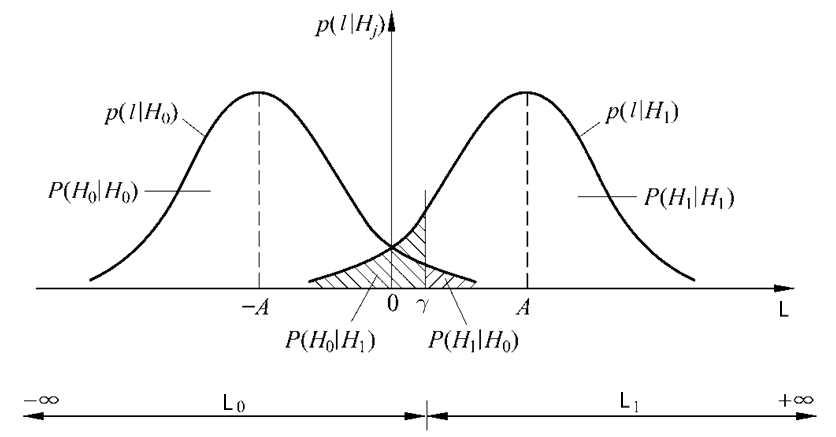
\includegraphics[scale=0.28]{detectionL}
\end{columns}
\end{frame}

\begin{frame}{判决概率的计算}
\begin{align*}
\lambda(\bm{x})=\frac{p(\bm{x}|H_1)}{p(\bm{x}|H_0)}\qquad \text{or}\qquad \lambda(\bm{\overline{x}})=\frac{p(\bm{\overline{x}}|H_1)}{p(\bm{\overline{x}}|H_0)}
\end{align*}
\centering $\Downarrow$
\begin{align*}
\ln(\lambda(\bm{x}))=\ln\left(\frac{p(\bm{x}|H_1)}{p(\bm{x}|H_0)}\right)\qquad \text{or}\qquad \ln(\lambda(\bm{\overline{x}}))=\ln\left(\frac{p(\bm{\overline{x}}|H_1)}{p(\bm{\overline{x}}|H_0)}\right)
\end{align*}
\centering $\Downarrow$
\begin{align*}
\textbf{最终统计量}\qquad l(\bm{x})\quad \text{or}\quad l(\bm{\overline{x}})
\end{align*}\\
~\\
\textbf{\textcolor{blue}{根据最终的统计量来计算各种判决概率}}
\end{frame}

\begin{frame}[shrink]{判决概率的计算步骤}
\textbf{\textcolor{blue}{计算基本原则: 根据化简后的最简判决表达式进行计算。}} 计算步骤如下:
\begin{enumerate}
	\item 推导贝叶斯检测准则的最简判决表达式。 \[l(\bm{x})\mathop{\gtrless}\limits_{H_0}^{H_1}\gamma \]
	\item 根据最简判决表达式, 计算各种假设下, 统计量的概率密度函数。
	\[p(l|H_0)\qquad p(l|H_1)\]
	\item 计算判决概率
	\begin{columns}
		\column{0.5\textwidth}
		\begin{align*}
		P(H_0|H_1)=\int_{-\infty}^{\gamma}p(l|H_1)dl\\
		P(H_1|H_0)=\int_{\gamma}^{\infty}p(l|H_0)dl\\
		P(H_1|H_1)=1-P(H_0|H_1)\\
		P(H_0|H_0)=1-P(H_1|H_0)
		\end{align*}
		\column{0.5\textwidth}
		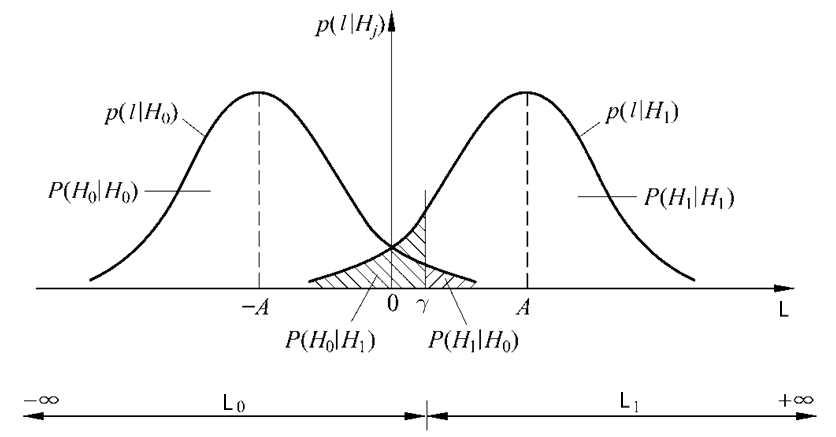
\includegraphics[scale=0.3]{detectionL}
	\end{columns}
\end{enumerate}
\end{frame}

\begin{frame}{贝叶斯准则例题3}
考虑以下信号检测问题:
\begin{align*}
H_0: x_k&=n_{k},   & k=1,2,\dots,N\\
H_1: x_k&=A+n_{k}, & k=1,2,\dots,N
\end{align*}
其中$n_{k}$是均值为零,方差为$\sigma_n^2$的高斯随机变量,  且不同采样时刻的加性噪声之间是相互统计独立的。请\\
\begin{enumerate}
	\item 请给出上述问题的贝叶斯检测准则。
	\item 当$N=1$时, 计算判决概率$P(H_1|H_1)$和$P(H_1|H_0)$。
	\item 当$N>1$时, 计算判决概率$P(H_1|H_1)$和$P(H_1|H_0)$。
\end{enumerate}
\end{frame}

\begin{frame}[shrink]{贝叶斯准则例题3: 解}
解: $N$次独立采样, 样本为$x_k(k=1,2,\cdots,N)$:
\begin{align*}
H_0: x_k&=n_k && k=1,2,\cdots,N\\
H_1: x_k&=A+n_k && k=1,2,\cdots,N
\end{align*}
\textbf{步骤1: 计算两个似然函数, 构建似然比}\\
由于$n$是高斯分布随机变量, 因此在$H_0$假设下, 第$k$次采样值$x_k$服从高斯分布,且均值为0, 方差为$\sigma_n^2$; 在$H_1$假设下, 第$k$次采样值$x_k$服从均值为$A$, 方差为$\sigma_n^2$的高斯分布。
\begin{align*}
p(x_k|H_0)&=\left(\frac{1}{2\pi\sigma_n^2}\right)^{1/2}\exp\left(-\frac{x_k^2}{2\sigma_n^2}\right)\implies p(\bm{x}|H_0)=\prod_{k=1}^{N}\left(\frac{1}{2\pi\sigma_n^2}\right)^{1/2}\exp\left(-\frac{x_k^2}{2\sigma_n^2}\right)\\
p(x_k|H_1)&=\left(\frac{1}{2\pi\sigma_n^2}\right)^{1/2}\exp\left(-\frac{(x_k-A)^2}{2\sigma_n^2}\right)\implies p(\bm{x}|H_1)=\prod_{k=1}^{N}\left(\frac{1}{2\pi\sigma_n^2}\right)^{1/2}\exp\left(-\frac{(x_k-A)^2}{2\sigma_n^2}\right)\\
\lambda(\bm{x})&=\frac{p(\bm{x}|H_1)}{p(\bm{x}|H_0)}=\exp\left(\frac{\sum\limits_{k=1}^{N}(x_k^2-(x_k-A)^2)}{2\sigma_n^2}\right)
\end{align*} 
\end{frame}

\begin{frame}[shrink]{贝叶斯准则例题3: 解续(1)}
\textbf{步骤2: 根据两个假设的先验概率和代价因子, 计算判决门限}
\[\eta\mathop{=}\limits^{def}\frac{P(H_0)(c_{10}-c_{00})}{P(H_1)(c_{01}-c_{11})} \]
\textbf{步骤3: 形成贝叶斯检测基本表达式}
\begin{align*}
\lambda(\bm{x})=\frac{p(\bm{x}|H_1)}{p(\bm{x}|H_0)}&\mathop{\gtrless}\limits_{H_0}^{H_1}\eta\\
\exp\left(\frac{\sum\limits_{k=1}^{N}(x_k^2-(x_k-A)^2)}{2\sigma_n^2}\right)&\mathop{\gtrless}\limits_{H_0}^{H_1}\eta
\end{align*} 
\textbf{步骤4: 化简, 形成贝叶斯检测判决表达式}
\begin{align*}
-NA^2+\sum\limits_{k=1}^{N}2Ax_k&\mathop{\gtrless}\limits_{H_0}^{H_1}2\sigma_n^2\ln\eta\implies \sum\limits_{k=1}^{N}x_k\mathop{\gtrless}\limits_{H_0}^{H_1}\frac{\sigma_n^2\ln\eta}{A}+\frac{NA}{2}\\
l(\bm{x})\mathop{=}^{def}\frac{1}{N}\sum\limits_{k=1}^{N}x_k&\mathop{\gtrless}\limits_{H_0}^{H_1}\frac{\sigma_n^2\ln\eta}{NA}+\frac{A}{2}\mathop{=}^{def}\gamma\\
\end{align*} 
\end{frame}

\begin{frame}[shrink]{贝叶斯准则例题3: 解续(2)}
经过上述化简, 信号检测的判决式由似然比检验的形式, 简化为检验统计量$l(x)$与检测门限$\gamma$相比较的形式, 形成贝叶斯检测判决表达式:
\[
l(\bm{x})\mathop{=}^{def}\frac{1}{N}\sum\limits_{k=1}^{N}x_k\mathop{\gtrless}\limits_{H_0}^{H_1}\frac{\sigma_n^2\ln\eta}{NA}+\frac{A}{2}\mathop{=}^{def}\gamma
\]
检验统计量$l(x)\mathop{=}\limits^{def}\frac{1}{N}\sum\limits_{k=1}^Nx_k$是观测信号$x_k(k=1,2,\dots,N)$的求和取平均值的结果, 即它是$x_k(k=1,2,\dots,N)$的函数,是一个随机变量。\\
因为高斯随机变量的线性组合还是高斯随机变量,  所以两种假设下的观测量$(l|H_0),(l|H_1)$也是服从高斯分布的随机变量。
\end{frame}

\begin{frame}[shrink]{贝叶斯准则例题3: 解续(3)}
$N$次独立采样, 样本为$x_k(k=1,2,\dots,N)$
\begin{align*}
&&n_k\sim\mathcal{N}(0,\sigma_n^2)\\ 
H_0 &:x_k=n_k   &(l|H_0)\sim\mathcal{N}(0,\frac{\sigma_n^2}{N})\\
H_1 &:x_k=A+n_k &(l|H_1)\sim\mathcal{N}(A,\frac{\sigma_n^2}{N})
\end{align*}
\begin{columns}
\column{0.4\textwidth}	
\textbf{贝叶斯检测判决表达式:}\\
\[
l(\bm{x})\mathop{=}^{def}\frac{1}{N}\sum\limits_{k=1}^{N}x_k\mathop{\gtrless}\limits_{H_0}^{H_1}\frac{\sigma_n^2\ln\eta}{NA}+\frac{A}{2}\mathop{=}^{def}\gamma
\]
\column{0.4\textwidth}
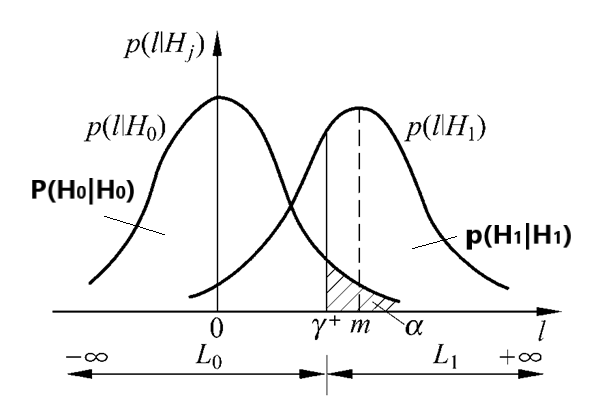
\includegraphics[scale=0.25]{mgt0}\\
\scriptsize
\textcolor{blue}{$p(l|H_j)(j=0,1)$: 假设$H_j$下观测信号的概率密度函数; $r^+=\frac{\sigma^2\ln\eta}{Nm}+\frac{m}{2}; \alpha=P(H_1|H_0)$}
\end{columns}
\end{frame}

\begin{frame}[shrink]{贝叶斯准则例题3: 性能分析---观测量$(l|H_0)$}
\[
\frac{1}{N}\sum\limits_{k=1}^{N}x_k\mathop{\gtrless}\limits_{H_0}^{H_1}\frac{\sigma_n^2\ln\eta}{NA}+\frac{A}{2}\mathop{=}\limits^{def}\gamma \qquad \textbf{统计量: }l(\bm{x})\mathop{=}\limits^{def}\frac{1}{N}\sum\limits_{k=1}^{N}x_k
\]
\textbf{假设$H_0$条件下, 统计量$l(x)$为高斯分布, 均值和方差分别为}
\begin{align*}
E[l|H_0]&=E\left[\frac{1}{N}\sum\limits_{k=1}^{N}(x_k|H_0)\right]=E\left[\frac{1}{N}\sum\limits_{k=1}^{N}n_k\right]=\frac{1}{N}\sum\limits_{k=1}^{N}E[n_k]=0\\
Var[l|H_0]&=E\left[(l|H_0-E(l|H_0))^2\right]=E\left[\left(\frac{1}{N}\sum\limits_{k=1}^{N}n_k\right)^2\right]\\
&=\frac{1}{N^2}\sum\limits_{k=1}^{N}E[n_k^2]=\frac{1}{N^2}\sum\limits_{k=1}^{N}\sigma_n^2=\frac{\sigma_n^2}{N}
\end{align*}
\textbf{因此, }$(l|H_0)\sim\mathcal{N}(0,\frac{\sigma_n^2}{N})$
\begin{align*}
p(l|H_0)=\left(\frac{1}{2\pi Var[l|H_0]}\right)^{1/2}\exp\left(-\frac{(l-E[l|H_0])^2}{2 Var[l|H_0]}\right)=\left(\frac{N}{2\pi\sigma_n^2}\right)^{1/2}\exp\left(-\frac{Nl^2}{2\sigma_n^2}\right)
\end{align*}
\end{frame}

\begin{frame}[shrink]{贝叶斯准则例题3: 性能分析---观测量$(l|H_0)$}
\[
\frac{1}{N}\sum\limits_{k=1}^{N}x_k\mathop{\gtrless}\limits_{H_0}^{H_1}\frac{\sigma_n^2\ln\eta}{NA}+\frac{A}{2}\mathop{=}\limits^{def}\gamma \qquad \textbf{统计量: }l(\bm{x})\mathop{=}\limits^{def}\frac{1}{N}\sum\limits_{k=1}^{N}x_k
\]
\begin{align*}
p(l|H_0)=\left(\frac{N}{2\pi\sigma_n^2}\right)^{1/2}\exp\left(-\frac{Nl^2}{2\sigma_n^2}\right)
\end{align*}
\begin{align*}
P(H_1|H_0)&=\int_{\gamma}^{\infty}p(l|H_0)dl\implies Q(u)=\int_{x}^{\infty}\left(\frac{1}{2\pi}\right)^{1/2}\exp\left(-\frac{u^2}{2}\right)du\\
&=\int_{\gamma}^{\infty}\left(\frac{N}{2\pi\sigma_n^2}\right)^{1/2}\exp\left(-\frac{Nl^2}{2\sigma_n^2}\right)dl\qquad \text{by } l=\frac{\sigma_nu}{\sqrt{N}}\\
&=\int_{\frac{\sqrt{N}\gamma}{\sigma_n}}^{\infty}\left(\frac{1}{2\pi}\right)^{1/2}\exp\left(-\frac{u^2}{2}\right)du\\
&=Q\left(\frac{\sqrt{N}\gamma}{\sigma_n}\right)=Q\left(\frac{\sqrt{N}\left(\frac{\sigma_n^2\ln\eta}{NA}+\frac{A}{2}\right)}{\sigma_n}\right)
\end{align*}
\end{frame}

\begin{frame}[shrink]{贝叶斯准则例题3: 性能分析---观测量$(l|H_0)$}
\[
\frac{1}{N}\sum\limits_{k=1}^{N}x_k\mathop{\gtrless}\limits_{H_0}^{H_1}\frac{\sigma_n^2\ln\eta}{NA}+\frac{A}{2}\mathop{=}\limits^{def}\gamma \qquad \textbf{统计量: }l(\bm{x})\mathop{=}\limits^{def}\frac{1}{N}\sum\limits_{k=1}^{N}x_k
\]
\begin{align*}
P(H_1|H_0)&=Q\left(\frac{\sqrt{N}\left(\frac{\sigma_n^2\ln\eta}{NA}+\frac{A}{2}\right)}{\sigma_n}\right)\\
&=Q\left(\frac{\sigma_n\ln\eta}{\sqrt{N}A}+\frac{\sqrt{N}A}{2\sigma_n}\right)&& \text{by }d^2=\frac{NA^2}{\sigma_n^2}\\
&=Q\left(\frac{\ln\eta}{d}+\frac{d}{2}\right)
\end{align*}
\end{frame}

\begin{frame}[shrink]{贝叶斯准则例题3: 性能分析---观测量$(l|H_1)$}
\[
\frac{1}{N}\sum\limits_{k=1}^{N}x_k\mathop{\gtrless}\limits_{H_0}^{H_1}\frac{\sigma_n^2\ln\eta}{NA}+\frac{A}{2}\mathop{=}\limits^{def}\gamma \qquad \textbf{统计量: }l(\bm{x})\mathop{=}\limits^{def}\frac{1}{N}\sum\limits_{k=1}^{N}x_k
\]
\textbf{假设$H_1$条件下, 统计量$l(x)$为高斯分布, 均值和方差分别为}
\begin{align*}
E[l|H_1]&=E\left[\frac{1}{N}\sum\limits_{k=1}^{N}(x_k|H_1)\right]=E\left[\frac{1}{N}\sum\limits_{k=1}^{N}(A+n_k)\right]=A+\frac{1}{N}\sum\limits_{k=1}^{N}E[n_k]=A\\
Var[l|H_1]&=E\left[(l|H_1-E(l|H_1))^2\right]=E\left[\left(\frac{1}{N}\sum\limits_{k=1}^{N}(A+n_k)-A\right)^2\right]\\
&=\frac{1}{N^2}\sum\limits_{k=1}^{N}E[n_k^2]=\frac{1}{N^2}\sum\limits_{k=1}^{N}\sigma_n^2=\frac{\sigma_n^2}{N}
\end{align*}
\textbf{因此, }$(l|H_1)\sim\mathcal{N}(A,\frac{\sigma_n^2}{N})$
\begin{align*}
p(l|H_1)=\left(\frac{1}{2\pi Var[l|H_1]}\right)^{1/2}\exp\left(-\frac{(l-E[l|H_1])^2}{2 Var[l|H_1]}\right)=\left(\frac{N}{2\pi\sigma_n^2}\right)^{1/2}\exp\left(-\frac{N(l-A)^2}{2\sigma_n^2}\right)
\end{align*}
\end{frame}

\begin{frame}[shrink]{贝叶斯准则例题3: 性能分析---观测量$(l|H_1)$}
\[
\frac{1}{N}\sum\limits_{k=1}^{N}x_k\mathop{\gtrless}\limits_{H_0}^{H_1}\frac{\sigma_n^2\ln\eta}{NA}+\frac{A}{2}\mathop{=}\limits^{def}\gamma \qquad \textbf{统计量: }l(\bm{x})\mathop{=}\limits^{def}\frac{1}{N}\sum\limits_{k=1}^{N}x_k
\]
\begin{align*}
p(l|H_1)=\left(\frac{N}{2\pi\sigma_n^2}\right)^{1/2}\exp\left(-\frac{N(l-A)^2}{2\sigma_n^2}\right)
\end{align*}
\begin{align*}
P(H_1|H_1)&=\int_{\gamma}^{\infty}p(l|H_1)dl\implies Q(u)=\int_{x}^{\infty}\left(\frac{1}{2\pi}\right)^{1/2}\exp\left(-\frac{u^2}{2}\right)du\\
&=\int_{\gamma}^{\infty}\left(\frac{N}{2\pi\sigma_n^2}\right)^{1/2}\exp\left(-\frac{N(l-A)^2}{2\sigma_n^2}\right)dl\qquad \text{by } l=\frac{\sigma_nu}{\sqrt{N}}+A\\
&=\int_{\frac{\sqrt{N}(\gamma-A)}{\sigma_n}}^{\infty}\left(\frac{1}{2\pi}\right)^{1/2}\exp\left(-\frac{u^2}{2}\right)du\\
&=Q\left(\frac{\sqrt{N}(\gamma-A}{\sigma_n}\right)=Q\left(\frac{\sqrt{N}\left(\frac{\sigma_n^2\ln\eta}{NA}-\frac{A}{2}\right)}{\sigma_n}\right)
\end{align*}
\end{frame}

\begin{frame}[shrink]{贝叶斯准则例题3: 性能分析---观测量$(l|H_1)$}
\[
\frac{1}{N}\sum\limits_{k=1}^{N}x_k\mathop{\gtrless}\limits_{H_0}^{H_1}\frac{\sigma_n^2\ln\eta}{NA}+\frac{A}{2}\mathop{=}\limits^{def}\gamma \qquad \textbf{统计量: }l(\bm{x})\mathop{=}\limits^{def}\frac{1}{N}\sum\limits_{k=1}^{N}x_k
\]
\begin{align*}
P(H_1|H_1)&=Q\left(\frac{\sqrt{N}\left(\frac{\sigma_n^2\ln\eta}{NA}-\frac{A}{2}\right)}{\sigma_n}\right)\\
&=Q\left(\frac{\sigma_n\ln\eta}{\sqrt{N}A}-\frac{\sqrt{N}A}{2\sigma_n}\right)&& \text{by }d^2=\frac{NA^2}{\sigma_n^2}\\
&=Q\left(\frac{\ln\eta}{d}-\frac{d}{2}\right)
\end{align*}
\end{frame}

\begin{frame}[shrink]{贝叶斯准则例题3(小结1)}
\begin{columns}
	\column{0.6\textwidth}
	$N$次独立采样, 样本为$x_k(k=1,2,\dots,N)$
	\begin{align*}
	&&n_k\sim\mathcal{N}(0,\sigma_n^2)\\ 
	H_0 &:x_k=n_k   &(l|H_0)\sim\mathcal{N}(0,\frac{\sigma_n^2}{N})\\
	H_1 &:x_k=A+n_k &(l|H_1)\sim\mathcal{N}(A,\frac{\sigma_n^2}{N})
	\end{align*}
	检验统计量$l(\bm{x})$, 归一化后, $(l|H_j)\sim\mathcal{N}(0,1)$
	\column{0.4\textwidth}
	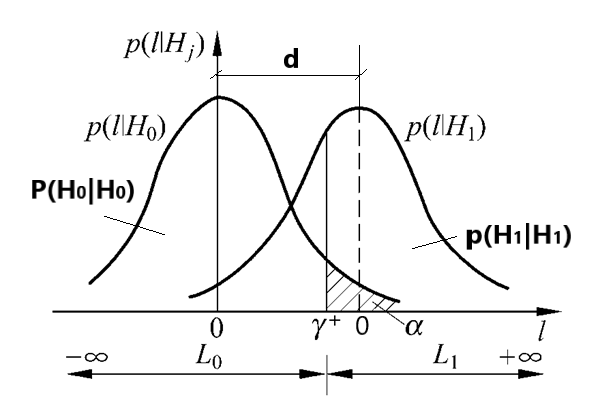
\includegraphics[scale=0.3]{0A}\\
	\scriptsize
	\textcolor{blue}{$p(l|H_j)(j=0,1)$: 假设$H_j$下观测信号的概率密度函数; $r^+=\frac{\ln\eta}{d}+\frac{d}{2}; \alpha=P(H_1|H_0)$}
\end{columns}
\[
\textbf{判决表达式: }\qquad l(\bm{x})\mathop{=}^{def}\frac{1}{N}\sum\limits_{k=1}^Nx_k\mathop{\gtrless}_{H_0}^{H_1}\frac{\sigma^2\ln\eta}{NA}+\frac{A}{2}\mathop{=}^{def}\gamma
\]

\textbf{判决概率:} (式中, 信噪比$d^2=\frac{NA^2}{\sigma^2}$)
\begin{align*}
P(H_1|H_0)&=Q\left(\frac{\ln\eta}{d}+\frac{d}{2}\right), &P(H_0|H_0)&=1-Q\left(\frac{\ln\eta}{d}+\frac{d}{2}\right)\\
P(H_1|H_1)&=Q\left(\frac{\ln\eta}{d}-\frac{d}{2}\right),
&P(H_0|H_1)&=1-Q\left(\frac{\ln\eta}{d}-\frac{d}{2}\right)
\end{align*}
\end{frame}

\begin{frame}{贝叶斯准则例题3(小结2)}
\begin{columns}
	\column{0.4\textwidth}
	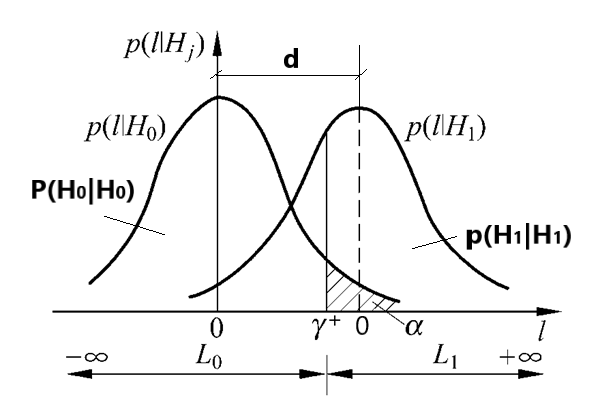
\includegraphics[scale=0.2]{0A}
	\scriptsize
	\textcolor{blue}{$p(l|H_j)(j=0,1)$: 假设$H_j$下观测信号的概率密度函数; $r^+=\frac{\ln\eta}{d}+\frac{d}{2}; \alpha=P(H_1|H_0)$}
	\column{0.4\textwidth}
	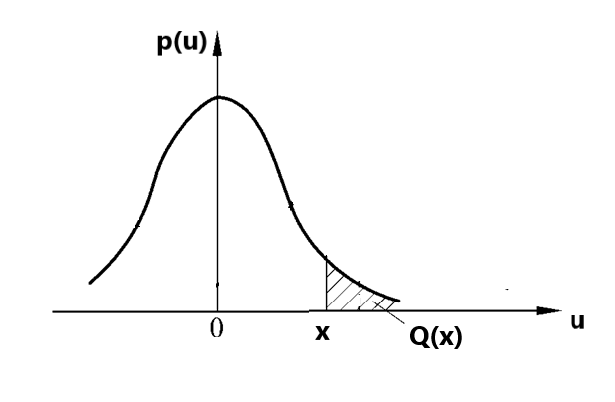
\includegraphics[scale=0.2]{Qx}
	\scriptsize
	\textcolor{red}{$Q(x)=\int_{x}^{\infty}\frac{1}{\sqrt{2\pi}}\exp(-\frac{u^2}{2})du$.}\\
	\textcolor{red}{$Q(x)$是单调递减函数, 其反函数: $Q^{-1}[\bullet]$}
\end{columns}

\bigskip

因为$P(H_1|H_0)=Q(\ln\eta/d+d/2) \implies \ln\eta/d=Q^{-1}[P(H_1|H_0)]-d/2$\\
这样有:
\begin{align*}
P(H_1|H_1)&=Q\left(\ln\eta/d-d/2\right)\\
&=Q[Q^{-1}[P(H_1|H_0)]-d/2-d/2]=Q[Q^{-1}[P(H_1|H_0)]-d]
\end{align*}
\colorbox{yellow}{这说明, 当给定$P(H_1|H_0)$时, $P(H_1|H_1)$随功率信噪比$(d^2=NA^2/\sigma^2)$单调增加。} 
\colorbox{green}{另一方面, 采样次数$N\uparrow\implies d\uparrow$, $p(l|H_0),p(l|H_1)$的间距$d\uparrow$,  检测性能$\uparrow$。} 
\end{frame}




